
%(BEGIN_QUESTION)
% Copyright 2012, Tony R. Kuphaldt, released under the Creative Commons Attribution License (v 1.0)
% This means you may do almost anything with this work of mine, so long as you give me proper credit

A type of heating system developed to provide a measure of safety and convenience for self-sufficient homes is an {\it external heater}, where fuel such as wood is burned at high temperature for short durations in an outdoor furnace, and the heat from that furnace stored in a large ``thermal reservoir'' of sand.  A fire is lit inside the furnace only once every few days, then the heat from that burn is transferred to the home by means of water pumped through heat exchangers:

$$\includegraphics[width=15.5cm]{i01017x01.eps}$$

Answer the following questions about this type of heating system:

\begin{itemize}
\item{} What advantages might there be with this design versus a furnace installed inside the home?
\vskip 5pt
\item{} Why is {\it sand} a good choice as a heat-storage medium inside the furnace structure?
\vskip 5pt
\item{} Is the heat storage in this system based on {\it specific heat} or {\it latent heat}?
\vskip 5pt
\item{} Is the heat transfer in this system (from heater to home) based on {\it specific heat} or {\it latent heat}?
\vskip 5pt
\item{} How may the home's temperature be thermostatically controlled?
\vskip 5pt
\item{} How to equip the system with an alarm prompting the user to light a new fire in the furnace?
\vskip 5pt
\item{} Calculate the enthalpy of the water as it enters the home (from the heater) at a temperature of 184 $^{o}$F.
\vskip 5pt
\item{} Calculate the enthalpy of the water as it leaves the home (on its way to the heater) at a temperature of 127 $^{o}$F.
\vskip 5pt
\item{} Calculate the rate of heat delivered to the home by this hot water assuming a water mass flow rate of 9.2 pounds per minute.
\end{itemize}

\underbar{file i01017}
%(END_QUESTION)





%(BEGIN_ANSWER)

\begin{itemize}
\item{} What advantages might there be with this design versus a furnace installed inside the home? {\it Safety (no fire hazard or smoke hazard inside the home), Efficiency (wood fires are very efficient and practically smokeless when burned at full intensity as is permitted with a heat-storage system like this), Convenience (the fire need not be tended for hours each day, but rather is lit and forgotten until the next fire needs to be lit)}
\vskip 5pt
\item{} Why is {\it sand} a good choice as a heat-storage medium inside the furnace structure? {\it Sand does not melt, freeze, corrode, or leak.  It has a high density and a reasonable heat capacity (approximately 0.19).}
\vskip 5pt
\item{} Is the heat storage in this system based on {\it specific heat} or {\it latent heat}?  {\it Since the sand does not change phase with the temperature of the furnace, this system is based on specific heat.}
\vskip 5pt
\item{} Is the heat transfer in this system (from heater to home) based on {\it specific heat} or {\it latent heat}? {\it Since the water does not boil in the heater, the transfer is strictly a function of specific heat.  If the water was boiled into steam and then sent to the house, the energy transfer would involve latent heat as well as specific heat!} 
\vskip 5pt
\item{} How may the home's temperature be thermostatically controlled? {\it A pump circulating the water between the furance and the house may be cycled by a thermostat control.}
\vskip 5pt
\item{} How to equip the system with an alarm prompting the user to light a new fire in the furnace? {\it A low-temperature alarm with a sensor embedded in the sand reservoir would suffice.}
\vskip 5pt
\item{} Calculate the enthalpy of the water as it enters the home (from the heater) at a temperature of 184 $^{o}$F.  {\it Enthalpy is simply the amount of heat energy released per pound of mass based on the temperature falling down to 32 $^{o}$F (0 $^{o}$C).  $Q = mc \Delta T$ = (1 lb)(1 BTU/lb-degF)(184 deg F $-$ 32 deg F) = 152 BTU.  Therefore, the enthalpy of the water entering the home is 152 BTU/lb.}
\vskip 5pt
\item{} Calculate the enthalpy of the water as it leaves the home (on its way to the heater) at a temperature of 127 $^{o}$F.  {\it Enthalpy is simply the amount of heat energy released per pound of mass based on the temperature falling down to 32 $^{o}$F (0 $^{o}$C).  $Q = mc \Delta T$ = (1 lb)(1 BTU/lb-degF)(127 deg F $-$ 32 deg F) = 95 BTU.  Therefore, the enthalpy of the water exiting the home is 95 BTU/lb.}
\vskip 5pt
\item{} Calculate the rate of heat delivered to the home by this hot water assuming a water mass flow rate of 9.2 pounds per minute.  {\it For every pound of heating water that circulates through the home, the amount of energy it delivers to the home is simply the difference between the incoming and outgoing enthalpy values.  152 BTU/lb $-$ 95 BTU/lb = 57 BTU/lb.  At a water flow rate of 9.2 pounds per minute, this equates to a heating rate of 524.4 BTU per minute, or 31,464 BTU per hour.}
\end{itemize}


%(END_ANSWER)





%(BEGIN_NOTES)

$$\includegraphics[width=15.5cm]{i01017x02.eps}$$

\vskip 20pt \vbox{\hrule \hbox{\strut \vrule{} {\bf Virtual Troubleshooting} \vrule} \hrule}

This question is a good candidate for a ``Virtual Troubleshooting'' exercise.  Presenting the diagram to students, you first imagine in your own mind a particular fault in the system.  Then, you present one or more symptoms of that fault (something noticeable by an operator or other user of the system).  Students then propose various diagnostic tests to perform on this system to identify the nature and location of the fault, as though they were technicians trying to troubleshoot the problem.  Your job is to tell them what the result(s) would be for each of the proposed diagnostic tests, documenting those results where all the students can see.

During and after the exercise, it is good to ask students follow-up questions such as:

\begin{itemize}
\item{} What does the result of the last diagnostic test tell you about the fault?
\item{} Suppose the results of the last diagnostic test were different.  What then would that result tell you about the fault?
\item{} Is the last diagnostic test the best one we could do?
\item{} What would be the ideal order of tests, to diagnose the problem in as few steps as possible?
\end{itemize}

%INDEX% Measurement, heat: conduction through a solid substance
%INDEX% Physics, heat and temperature: desuperheating

%(END_NOTES)


